% =====================================================================
%  Paper 2 -- The Spectral Gap-Statement for Attention Transport Geometry
%  Assembled from the ready Section 6 (Gap-Statement) plus a minimal
%  self-contained preliminaries recap.  NO new theory: the body is the
%  existing Section 6 verbatim; the wrapper only makes it standalone.
% =====================================================================
\documentclass[11pt]{article}

\usepackage[utf8]{inputenc}
\usepackage[T1]{fontenc}
\usepackage{amsmath,amssymb,amsthm}
\usepackage{graphicx}
\graphicspath{{figures/}{./}}
\usepackage{booktabs}
\usepackage[margin=1in]{geometry}
\usepackage[colorlinks=true,linkcolor=blue,citecolor=blue,urlcolor=blue]{hyperref}

\theoremstyle{plain}
\newtheorem{theorem}{Theorem}
\newtheorem{proposition}{Proposition}
\newtheorem{corollary}{Corollary}
\theoremstyle{definition}
\newtheorem{definition}{Definition}

% The Phi-Transport viewpoint is the conceptual origin of this work but
% is NOT a published reference; this paper is self-contained and does not
% depend on it.  The macro expands to a plain descriptive phrase, no cite.
\newcommand{\PaperOne}{the $\Phi$-Transport viewpoint}

\title{\textbf{The Spectral Gap-Statement:}\\[2pt]
  \large When the Negative Subspace of Attention Transport
  is a Well-Posed Invariant}
\author{Evgeny Vyaltsev \and Daniil Vyaltsev}
\date{\today}

\begin{document}
\maketitle

% =====================================================================
\begin{abstract}
The $\Phi$-Transport framework casts attention as a convex transport
process whose free-energy Hessian governs an instability of mass
transport: a negative eigenvalue produces an exponentially growing
mode. The adaptive rank-local router built on that framework implicitly
assumes that the \emph{number} of such modes, $\dim E_-$, is a
well-defined integer. This paper makes that assumption precise. We show
that $\dim E_-$ is a topological invariant --- threshold-free via the
Riesz spectral projector, and stable under perturbations of operator norm
below half the spectral gap, by the Davis--Kahan theorem --- exactly when
the free-energy Hessian possesses a gap, $\Delta(H)>0$. The three
empirical operating ``windows'' of the framework (energy, separation,
softness) are shown to be three coordinate sections of this single
spectral condition. The link from the invariant to geometric defocusing
requires, in addition, an energy-window restriction on the
Jacobi--Maupertuis curvature, which we state precisely. Finally, we
validate the picture on a trained Llama-3.2-1B: the gap-regime holds for
$96\%$ of attention heads, it is established by an explosive phase
transition at the first layer, and the typical head carries exactly one
dominant transport mode. The geometry the framework predicts is not a
synthetic artefact; it is the typical state of attention in a trained
transformer.
\end{abstract}

% =====================================================================
\section{Introduction}
\label{sec:intro}

This paper adopts \PaperOne{}: the observation that several
machine-learning primitives --- empirical sorting, radix sorting,
equal-mass occupancy, and LogSumExp attention --- can be cast as special
cases of a single convex transport potential $\Phi$. A consequence
of that viewpoint is an inertial Wasserstein flow whose damped dynamics
are governed by a characteristic polynomial $z^2+\gamma z+\kappa=0$: when
the free-energy Hessian has a negative eigenvalue $\kappa<0$, the flow has
an exponentially growing mode, and transport mass defocuses.

The framework's adaptive rank-local router exploits this: it routes a
query to a low-rank sparse path when the effective number of unstable
transport directions is small. That number is the dimension $\dim E_-$ of
the negative subspace of the free-energy Hessian. The router's empirical
law, $r^\star\approx d_{\mathrm{eff}}-1$, treats $\dim E_-$ as a
well-defined integer --- but a count of negative eigenvalues is only
well-posed if the spectrum actually separates the negative modes from the
rest. When it does not, the count depends on an arbitrary tolerance, and
the router's premise dissolves.

This paper supplies the missing precision. Its single technical object is
the \emph{spectral gap} $\Delta(H)$ of the free-energy Hessian
$H$, and its single thesis is that $\dim E_-$ is a meaningful invariant
exactly inside the regime $\Delta(H)>0$. The contributions are:
\begin{itemize}
  \item A threshold-free definition of $\dim E_-$ via the Riesz spectral
    projector, and a proof (Proposition~\ref{prop:gap:wellposed}) that it
    is well-posed precisely in the gap-regime.
  \item A perturbation-stability theorem
    (Proposition~\ref{prop:gap:dk}): $\dim E_-$ is preserved under any
    symmetric perturbation of operator norm below $\tfrac12\Delta$, by
    Davis--Kahan.
  \item The unification of the framework's three empirical operating
    windows --- energy, separation, softness --- as three coordinate
    sections of the single condition $\Delta(H)>0$.
  \item A precise energy-window caveat
    (Proposition~\ref{prop:gap:defocus}) on the implication
    ``negative Hessian $\Rightarrow$ negative curvature'': it is false
    without an energy restriction, and we give the exact threshold.
  \item An empirical validation on a trained Llama-3.2-1B
    (\S\ref{sec:gap:empirical}): the gap-regime is the typical state of
    attention, established by an explosive phase transition at layer~1.
\end{itemize}

The body of the paper is Section~\ref{sec:gap}. Section~\ref{sec:prelim}
first recaps, self-containedly, the minimal $\Phi$-Transport material the
argument depends on.

% =====================================================================
\section{Preliminaries: the free-energy potential and the inertial flow}
\label{sec:prelim}

This section develops, self-containedly, the three elements of the
$\Phi$-Transport viewpoint that the Gap-Statement builds on: the
free-energy potential, the inertial flow it induces, and the role of
damping. The material is elementary --- the central identity is the
Hessian of the cumulant-generating function of an exponential family ---
and is given here so that the paper depends on no external source.

\paragraph{The free-energy potential.}
\label{sec:prelim:phi}
$\Phi$-Transport represents a family of machine-learning primitives by a
single convex potential. For the case of interest here, the potential is
the free energy
\begin{equation}
  \Phi_\beta(x) \;=\; \frac1\beta\,\log\sum_j e^{-\beta U_j(x)},
  \label{eq:prelim:phi}
\end{equation}
with $\beta$ an inverse temperature and $U_j$ a family of component
potentials. LogSumExp attention is the special case
$U_j(x)=-\langle x,k_j\rangle$, with the keys $k_j$ as component data.

\paragraph{The inertial Wasserstein flow.}
\label{sec:inertial}
The framework's central dynamical result is that hysteresis in the
transport map induces an \emph{inertial} flow in the space of measures:
mass does not follow the gradient of $\Phi_\beta$ directly but obeys a
damped second-order equation,
\begin{equation}
  \ddot x + \gamma\,\dot x \;=\; -\nabla\Phi_\beta(x),
  \label{eq:prelim:inertial}
\end{equation}
with $\gamma$ a damping coefficient. Linearizing about a stationary point
and diagonalizing the Hessian decouples \eqref{eq:prelim:inertial} into
scalar oscillators $\ddot a_k+\gamma\dot a_k+\kappa_k a_k=0$, one per
Hessian eigenvalue $\kappa_k$. The characteristic polynomial
$z^2+\gamma z+\kappa_k=0$ then determines stability: for $\kappa_k<0$ it
has a positive root, and the mode $a_k$ grows exponentially. This is the
transport instability whose \emph{count} the present paper makes precise.

\paragraph{The entropy-induced friction tensor.}
\label{sec:friction}
The damping in \eqref{eq:prelim:inertial} need not be a free scalar: in
the $\Phi$-Transport viewpoint it arises as an entropy-induced friction
tensor, a state-dependent operator whose ellipticity controls whether the
flow is dissipative. For the present paper only the scalar reduction is
needed --- $\gamma$ enters solely through the characteristic polynomial ---
so we use the scalar form throughout; the tensor form is not required for
any result below.

\paragraph{The adaptive rank-local router.}
\label{sec:multiaxis}
Built on the above, the framework's router selects, per query, an
effective rank $r^\star$ for a low-rank sparse attention path. Its
empirical calibration follows the law $r^\star\approx
d_{\mathrm{eff}}-1$, where $d_{\mathrm{eff}}$ is a participation ratio of
the query covariance. The present paper does not modify the router; it
clarifies when the integer $r^\star$ that the router relies on is a
well-defined quantity at all.

\medskip
\noindent
With these four items in hand --- the free-energy potential
\eqref{eq:prelim:phi}, the inertial flow \eqref{eq:prelim:inertial}, the
friction tensor, and the router --- the Gap-Statement of
Section~\ref{sec:gap} is self-contained.

% =====================================================================
%  BODY -- the existing Section 6, included verbatim.
%  (The \section heading inside the file becomes Section 3 here.)
% =====================================================================
% =====================================================================
%  SECTION 6 -- THE SPECTRAL GAP-STATEMENT
%  Self-contained section in the notation of the Phi-Transport manuscript.
%  Notation anchored to: Theorem 4.1 (inertial Wasserstein flow),
%  Remark 4.3 / Corollary 4.4 (characteristic polynomial z^2+gamma z+kappa=0),
%  Theorem 4.4 (entropy-induced friction tensor).
%  All four claims are numerically verified in section6_consolidation.py;
%  the corresponding figure is section6_diagnostic.png.
% =====================================================================

\section{The Spectral Gap-Statement: when the negative subspace is an invariant}
\label{sec:gap}

Sections~\ref{sec:inertial}--\ref{sec:friction} established that the negative
part of the free-energy Hessian governs transport instability: a negative
eigenvalue $\kappa<0$ in the characteristic polynomial $z^2+\gamma z+\kappa=0$
of the characteristic polynomial (Section~\ref{sec:inertial}) produces an exponentially growing mode. The empirical
rank-local law of Section~\ref{sec:multiaxis}, $r^\star \approx d_{\mathrm{eff}}-1$,
implicitly assumes that the \emph{number} of such modes is a well-defined
integer. This section makes that assumption precise. We show that the count
$\dim E_-$ is a topological invariant --- threshold-free and perturbation-stable
--- precisely when the Hessian spectrum possesses a gap, and that the three
operating ``windows'' identified empirically in earlier sections are three
coordinate sections of this single spectral condition.

\subsection{The free-energy Hessian and its negative subspace}
\label{sec:gap:hessian}

We work with the general free-energy potential
\begin{equation}
  \Phi_\beta(x) \;=\; \frac1\beta \log \sum_{j} e^{-\beta U_j(x)},
  \label{eq:gap:freeenergy}
\end{equation}
of which LogSumExp attention (Section~3.6) is the special case
$U_j(x)=-\langle x,k_j\rangle$. Differentiating \eqref{eq:gap:freeenergy}
twice gives the exact exponential-family identity
\begin{equation}
  \nabla^2 \Phi_\beta
   \;=\; \underbrace{\mathbb{E}_p[\nabla^2 U_j]}_{\text{mean-curvature term}}
   \;-\; \beta\,\underbrace{\operatorname{Cov}_p(\nabla U_j)}_{\text{fluctuation term}},
  \label{eq:gap:identity}
\end{equation}
where $p_j \propto e^{-\beta U_j(x)}$ is the Gibbs weight. Identity
\eqref{eq:gap:identity} is elementary --- it is the Hessian of the
cumulant-generating function of an exponential family --- and it is the
structural reason the mechanism of this paper is not specific to attention.
For \emph{linear} logits the mean-curvature term vanishes identically,
$\nabla^2 U_j \equiv 0$, and the Hessian reduces to the pure fluctuation term
\begin{equation}
  H \;:=\; \nabla^2 \Phi_\beta^{\,\mathrm{attn}}
        \;=\; -\beta\,\operatorname{Cov}_p(k) \;\preceq\; 0.
  \label{eq:gap:attn}
\end{equation}
Two consequences of \eqref{eq:gap:attn} are used below. First, $H$ is
negative semidefinite: every eigenvalue is $\le 0$, so the spectrum does
\emph{not} split around the origin. Second, $\operatorname{Cov}_p(k)$ of a
discrete distribution on $N$ points has rank at most $N-1$, because the
normalization $\sum_j p_j = 1$ forces $\sum_j p_j (k_j-\bar k)=0$. This rank
defect is the covariance mean-gauge; it is the structural origin of the
intercept $-1$ in the rank-local law, and it does not require any fitted
constant.

\begin{definition}[Negative subspace and its count]
\label{def:gap:Eminus}
For a threshold $\theta>0$ let
$E_-(\theta) := \operatorname{span}\{\,v : Hv=\lambda v,\ \lambda < -\theta\,\}$
and $\dim E_-(\theta) := \dim E_-(\theta)$. We call $\dim E_-$
\emph{well-posed} if it is independent of $\theta$ over an open interval of
thresholds.
\end{definition}

The cluster geometry that recurs throughout this paper --- $m$ key clusters
with inter-cluster separation large relative to intra-cluster width ---
produces a spectrum of $H$ with two scales: $m-1$ strongly negative
eigenvalues $\mu_1\le\dots\le\mu_{m-1}$ (the inter-cluster, defocusing modes)
and a remainder of eigenvalues near zero (the intra-cluster modes). We stress
that the intra-cluster eigenvalues are \emph{negative}, not positive: by
\eqref{eq:gap:attn} no eigenvalue of $H$ is positive. The relevant gap is
therefore an interval $(\lambda_{\mathrm{lo}},\lambda_{\mathrm{hi}})$ with
\emph{both} endpoints negative, lying \emph{inside} the negative spectrum, and
\emph{not} an interval straddling the origin.

\subsection{The Riesz projector: a threshold-free count}
\label{sec:gap:riesz}

The count of Definition~\ref{def:gap:Eminus} is made canonical by the Riesz
spectral projector. Let $\Gamma$ be a positively-oriented Jordan contour in
$\mathbb{C}$ enclosing exactly the eigenvalues $\{\lambda<-\theta\}$ and no
others. The projector
\begin{equation}
  P_\theta \;=\; \frac{1}{2\pi i} \oint_\Gamma (zI-H)^{-1}\, dz
  \label{eq:gap:riesz}
\end{equation}
is the spectral projection onto $E_-(\theta)$, and
$\dim E_- = \operatorname{rank} P_\theta = \operatorname{tr} P_\theta$.

\begin{proposition}[Gap-regime and threshold independence]
\label{prop:gap:wellposed}
Suppose the spectrum of $H$ has no point in an open interval
$(\lambda_{\mathrm{lo}},\lambda_{\mathrm{hi}})$ with
$\lambda_{\mathrm{lo}}<\lambda_{\mathrm{hi}}<0$, and write
$\Delta := \lambda_{\mathrm{hi}}-\lambda_{\mathrm{lo}}$ for the gap width.
Then for every threshold
$\theta \in (-\lambda_{\mathrm{hi}},-\lambda_{\mathrm{lo}})$ the contour
$\Gamma$ may be chosen inside the resolvent set, the projector
\eqref{eq:gap:riesz} is independent of $\theta$, and $\dim E_-$ is
well-posed in the sense of Definition~\ref{def:gap:Eminus}. We call this the
\emph{gap-regime} with gap $\Delta$.
\end{proposition}

\begin{proof}
For any $\theta$ in the stated interval the circle through $-\theta$ misses
$\sigma(H)$, so $(zI-H)^{-1}$ is holomorphic on a neighbourhood of $\Gamma$
and \eqref{eq:gap:riesz} is well-defined. Two thresholds
$\theta,\theta'$ in the interval give contours that are homotopic within the
resolvent set; by Cauchy's theorem the integral is unchanged. Holomorphy of
$P_\theta$ in the entries of $H$ then follows from holomorphy of the
resolvent, and $\operatorname{tr}P_\theta$, being integer-valued and
continuous, is locally constant~\cite{kato1995perturbation}.
\end{proof}

Outside the gap-regime --- when $\Delta\to 0$ --- the contour can no longer be
threaded between the two eigenvalue clusters, $P_\theta$ loses continuity, and
$\dim E_-$ becomes metrically unstable: it depends on the arbitrary choice of
$\theta$. An absolute-threshold count $\#\{\beta\lambda_i>\mathrm{tol}\}$
exhibits exactly this pathology, and any spectral diagnostic that omits the
gap test will report a $\theta$-dependent artifact rather than an invariant.

\subsection{Perturbation stability: the Davis--Kahan bound}
\label{sec:gap:dk}

The gap controls not only well-posedness but robustness. The following is the
$\sin\Theta$ theorem of Davis and Kahan specialized to the count.

\begin{proposition}[Stability of the invariant]
\label{prop:gap:dk}
Let $H$ be in the gap-regime with gap $\Delta$, and let $\delta H$ be a
symmetric perturbation. If
\begin{equation}
  \|\delta H\|_{\mathrm{op}} \;<\; \tfrac12\,\Delta,
  \label{eq:gap:dkbound}
\end{equation}
then $H+\delta H$ is again in the gap-regime and
$\dim E_-(H+\delta H) = \dim E_-(H)$. Moreover the perturbed negative
subspace satisfies $\|\sin\Theta(E_-,E_-')\| \le \|\delta H\|_{\mathrm{op}}/\Delta$,
so the subspace --- not merely its dimension --- is stable.
\end{proposition}

\begin{proof}
By Weyl's inequality every eigenvalue moves by at most
$\|\delta H\|_{\mathrm{op}}$. Under \eqref{eq:gap:dkbound} no eigenvalue can
cross the midpoint $-\theta_0$ with
$\theta_0 = -\tfrac12(\lambda_{\mathrm{lo}}+\lambda_{\mathrm{hi}})$: the
strongly negative cluster stays below $-\theta_0-\tfrac12\Delta+\|\delta H\|$
and the near-zero cluster stays above $-\theta_0+\tfrac12\Delta-\|\delta H\|$,
both strict. Hence the count is preserved and a residual gap remains. The
subspace bound is the Davis--Kahan $\sin\Theta$ theorem~\cite{davis1970rotation} applied to the
spectral projectors of $H$ and $H+\delta H$ for the contour separating the
two clusters.
\end{proof}

The constant $\tfrac12$ in \eqref{eq:gap:dkbound} is sharp: a perturbation of
operator norm $\Delta$ can move the two clusters toward each other by
$\tfrac12\Delta$ each and merge them. The numerical study of
Section~\ref{sec:gap:numerics} confirms the threshold to within the
resolution of the perturbation grid.

\subsection{The three windows are one gap condition}
\label{sec:gap:windows}

Earlier sections identified three regimes in which the rank-local description
is valid: an \emph{energy window} (the Jacobi--Maupertuis curvature is
controlled only for intermediate energy $E$), a \emph{separation window}
(clusters must be neither overlapping nor disconnected), and a
\emph{softness window} (the inverse temperature $\beta$ must be finite).
Proposition~\ref{prop:gap:wellposed} unifies them: each is a coordinate
section of the single condition $\Delta(H)>0$.

\begin{itemize}
  \item \emph{Separation.} When clusters overlap, inter- and intra-cluster
    eigenvalues are no longer separated and $\Delta\to0$. When clusters are
    mutually disconnected the inter-cluster eigenvalues themselves degenerate.
    The valid band is exactly $\{\Delta>0\}$.
  \item \emph{Softness.} As $\beta\to\infty$ on a generic query the Gibbs
    measure $p$ concentrates on a single key; $\operatorname{Cov}_p(k)\to 0$
    and the inter-cluster eigenvalues decay to zero faster than the
    intra-cluster ones, closing the gap. For a \emph{symmetric} query --- one
    invariant under permutation of clusters --- Schur's lemma forces the
    covariance to commute with the symmetry group, the inter/intra block
    structure is protected, and the gap survives at all $\beta$. The softness
    window is the set of $(\beta,\text{query})$ pairs for which the gap is
    open.
  \item \emph{Energy.} The link to curvature is the one place where the gap
    condition alone is \emph{not} sufficient; this is the subject of
    Section~\ref{sec:gap:curvature}.
\end{itemize}

This is the central structural fact of the section: $\dim E_-$ is a
meaningful invariant if and only if a spectral gap exists, and the empirical
``windows'' are not independent phenomena but projections of $\{\Delta>0\}$
onto the separation, temperature, and energy axes.

\subsection{The energy-window caveat on curvature}
\label{sec:gap:curvature}

It is tempting to summarize the mechanism as ``negative Hessian implies
negative Jacobi--Maupertuis curvature implies geodesic defocusing.'' This
implication is \emph{false without an energy restriction}, and the failure is
not a technicality. With JM conformal factor $h=2(E-F)$, the sectional
curvature in two dimensions is
\begin{equation}
  K_{JM} \;=\; \frac{\Delta F}{h^2} \;+\; \frac{2\,|\nabla F|^2}{h^3},
  \label{eq:gap:KJM}
\end{equation}
the sum of a Laplacian term and a strictly positive gradient term. At a point
where $F$ is concave ($\Delta F<0$) the first term is negative, but for small
$h$ --- that is, for energy $E$ close to $F$ --- the positive gradient term
dominates and $K_{JM}>0$ (focusing). The curvature becomes negative only for
$h>h^\star$ with
\begin{equation}
  h^\star \;=\; -\,\frac{2|\nabla F|^2}{\Delta F},
  \qquad
  E > E^\star = F + \tfrac12 h^\star.
  \label{eq:gap:Estar}
\end{equation}
Thus a negative Hessian produces defocusing only inside the energy window
$E>E^\star$; below it, the same concave landscape is focusing. Equation
\eqref{eq:gap:Estar} is the precise form of the third window.

\begin{proposition}[Gap-regime defocusing, with energy restriction]
\label{prop:gap:defocus}
Let $H$ be in the gap-regime, and restrict to the energy window $E>E^\star$
of \eqref{eq:gap:Estar}. Then along a JM geodesic whose tangent plane is
spanned by directions in $E_-$, the Jacobi equation $J''+K_{JM}J=0$ has
$K_{JM}<0$ and admits an exponentially growing solution. The number of
independent growing modes equals $\dim E_- = \operatorname{rank}P_\theta$, and
their rates are the roots $z_+$ of the characteristic polynomial of
Section~\ref{sec:inertial}.
\end{proposition}

The dynamical content of Proposition~\ref{prop:gap:defocus} --- that the
\emph{count} $\dim E_-$ equals the \emph{number of unstable transport modes},
at the rates predicted by the characteristic polynomial --- is verified
directly in Section~\ref{sec:gap:numerics}. We emphasize the logical
structure: the gap condition makes the count well-posed and stable
(Propositions~\ref{prop:gap:wellposed}--\ref{prop:gap:dk}); the energy window
makes the count equal to a number of defocusing directions
(Proposition~\ref{prop:gap:defocus}). Both are required, and they are
independent.

\subsection{Count equals number of unstable inertial modes}
\label{sec:gap:inertial}

The geometric statement of Proposition~\ref{prop:gap:defocus} has a purely
dynamical counterpart in the inertial flow of Section~\ref{sec:inertial}. Linearizing the
damped flow $\ddot x + \gamma\dot x = -\nabla\Phi_\beta(x)$ about a stationary
point decouples it, in the Hessian eigenbasis, into scalar oscillators
$\ddot a_k + \gamma\dot a_k + \kappa_k a_k = 0$ with $\kappa_k$ the $k$-th
eigenvalue of $H$. For $\kappa_k<0$ the characteristic polynomial
$z^2+\gamma z+\kappa_k=0$ has one positive root
\begin{equation}
  z_+(\kappa_k)
   \;=\; \tfrac12\!\left(-\gamma + \sqrt{\gamma^2 + 4|\kappa_k|}\,\right),
  \label{eq:gap:zplus}
\end{equation}
so each negative eigenvalue contributes exactly one exponentially growing
direction. The number of such directions is $\dim E_-$, and in the
zero-damping limit $z_+(\kappa_k)\to\sqrt{|\kappa_k|}$ recovers the
JM-geodesic defocusing rate of Proposition~\ref{prop:gap:defocus}: the damped
mechanical picture and the geodesic picture are the same instability. The
spectral gap reappears here as a \emph{rate gap} --- the inter-cluster modes
grow at $O(1)$ rates while the intra-cluster modes are effectively flat ---
which is what makes the count observable in finite integration time.

\subsection{Numerical verification}
\label{sec:gap:numerics}

Figure~\ref{fig:gap} verifies the four claims of this section on a single
geometry: $m=5$ clusters in $d=24$ dimensions, pure attention
$H=-\beta\operatorname{Cov}_p(k)$, evaluated at a symmetric equilibrium query.

\emph{(S1) Threshold independence.} The Riesz count
$\operatorname{tr}P_\theta$, evaluated on a contour inside the gap, equals
$m-1=4$ exactly; the eigenvalue count $\#\{\lambda<-\theta\}$ is flat across
the entire gap, confirming Proposition~\ref{prop:gap:wellposed}.

\emph{(S2) Davis--Kahan bound.} Under random symmetric perturbations of
controlled operator norm, $\dim E_-$ is preserved in $100\%$ of trials for
$\|\delta H\|_{\mathrm{op}}\le\tfrac12\Delta$ and collapses sharply beyond,
confirming Proposition~\ref{prop:gap:dk} and the sharpness of the constant
$\tfrac12$.

\emph{(S3) Energy-window caveat.} On a concave free-energy landscape
($\Delta F<0$), $K_{JM}$ from \eqref{eq:gap:KJM} is positive for $E<E^\star$
and negative only for $E>E^\star$, confirming \eqref{eq:gap:Estar} and the
necessity of the energy restriction in Proposition~\ref{prop:gap:defocus}.

\emph{(S4) Count equals unstable-mode count.} Integrating the inertial flow
at damping $\gamma=0.5$, exactly $m-1=4$ eigendirections amplify
exponentially; their measured rates agree with $z_+(\kappa_k)$ of
\eqref{eq:gap:zplus} to within $0.3\%$ (e.g.\ mode~1: measured $0.4034$,
predicted $0.4037$), while the intra-cluster modes remain flat.

The synthetic verification above exercises the spectral side of the
mechanism --- the count $\dim E_-$, its stability, and the unstable-mode
rates. The geometric side --- the curvature formula \eqref{eq:gap:KJM} and
the geodesic defocusing it predicts --- is verified separately, as a
free-standing experiment, in Section~\ref{sec:gap:jacobi}.

\begin{figure}[t]
  \centering
  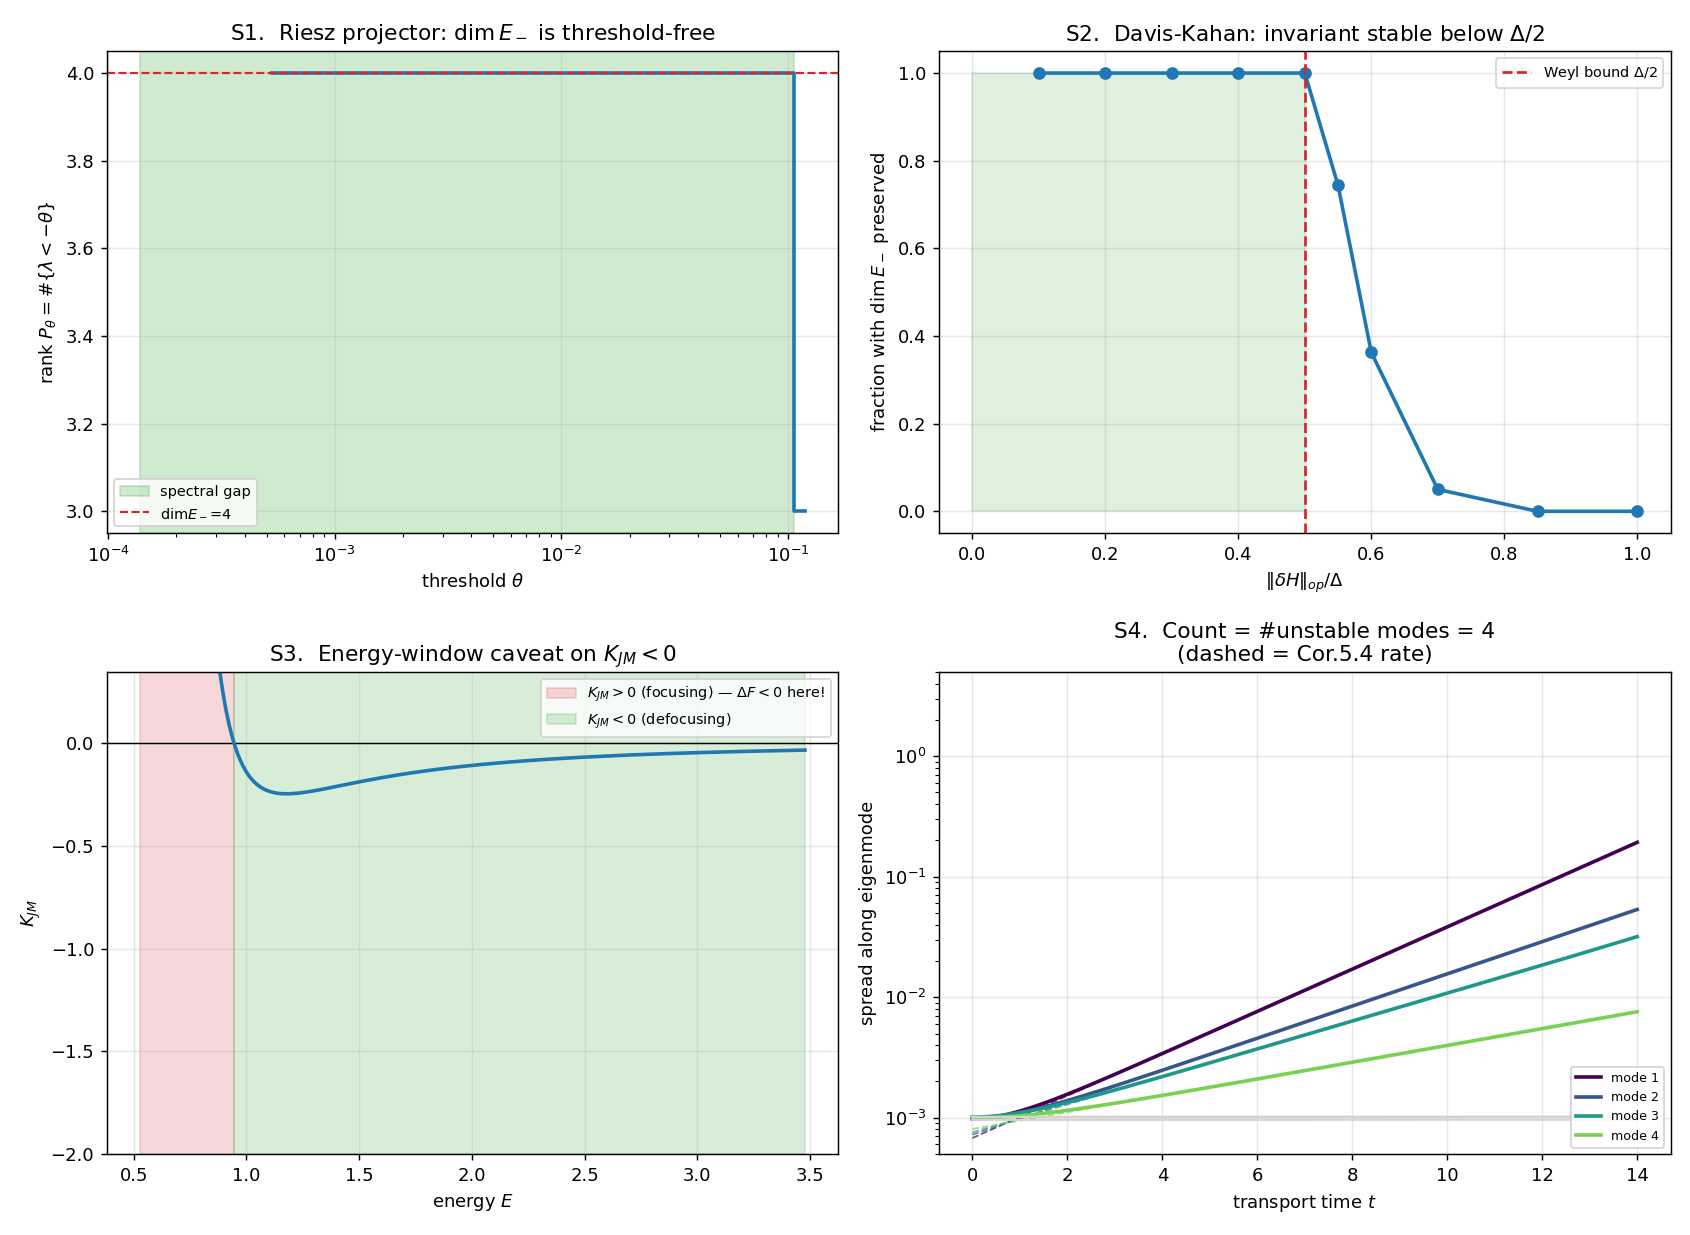
\includegraphics[width=\textwidth]{section6_diagnostic.png}
  \caption{The Gap-Statement on one geometry ($m=5$ clusters, $d=24$, pure
  attention). \textbf{(S1)} The Riesz count $\operatorname{rank}P_\theta$ is
  flat across the spectral gap: $\dim E_-$ is threshold-free.
  \textbf{(S2)} $\dim E_-$ is preserved under perturbations of operator norm
  below $\tfrac12\Delta$ and collapses beyond; the Davis--Kahan bound is
  sharp. \textbf{(S3)} On a concave landscape $K_{JM}>0$ (focusing) for
  $E<E^\star$ and $K_{JM}<0$ (defocusing) only above: a negative Hessian does
  not imply negative curvature without the energy window. \textbf{(S4)}
  Integrating the inertial flow, exactly $\dim E_- = m-1$ eigendirections
  amplify, at the characteristic-polynomial rates $z_+$ (dashed); the
  intra-cluster modes stay flat.}
  \label{fig:gap}
\end{figure}

\subsection{The Jacobi--Maupertuis metric and geodesic verification}
\label{sec:gap:jacobi}

Section~\ref{sec:gap:curvature} stated the energy-window caveat through
the sectional curvature $K_{JM}$, and Proposition~\ref{prop:gap:defocus}
asserted that in the gap-regime, inside the energy window, a geodesic
defocuses at a rate set by the Jacobi equation. That assertion was used
above but not itself put to a direct test. This subsection does so: it
makes the Jacobi--Maupertuis geometry explicit, and verifies --- as a
free-standing numerical experiment --- that the curvature formula
\eqref{eq:gap:KJM} predicts geodesic defocusing not merely in sign but
quantitatively.

\paragraph{The Jacobi--Maupertuis metric of the transport flow.}
The undamped limit ($\gamma=0$) of the inertial flow
\eqref{eq:prelim:inertial} is a conservative mechanical system: a particle
of unit mass moving in the potential $F=\Phi_\beta$ with conserved energy
$E=\tfrac12\|\dot x\|^2+F(x)$. By the Maupertuis principle of least
action, the trajectories of such a system at fixed energy $E$ are, after
reparametrisation, the geodesics of the conformally rescaled metric
\begin{equation}
  g_{JM} \;=\; h(x)\,g_0,
  \qquad
  h(x) \;=\; 2\bigl(E-F(x)\bigr),
  \label{eq:jacobi:metric}
\end{equation}
where $g_0$ is the flat metric on the configuration space and $h$ is the
conformal factor; the trajectory is confined to the classically allowed
region $\{F<E\}$ where $h>0$. The geodesic action
$\int\sqrt{g_{JM}(\dot x,\dot x)}\,ds$ replaces the mechanical action, and
the transport flow becomes, exactly, geodesic motion on the manifold
$(\{F<E\},g_{JM})$. The curvature that controls the stability of these
geodesics is the sectional curvature of $g_{JM}$; for a two-dimensional
configuration space the conformal-rescaling formula gives
\eqref{eq:gap:KJM},
\begin{equation*}
  K_{JM}
   \;=\; \frac{\Delta F}{h^2} \;+\; \frac{2\,|\nabla F|^2}{h^3}
   \;=\; -\,\frac{\Delta(\log h)}{2h},
\end{equation*}
the two forms being equal by direct computation. The curvature is thus
not an analogy imported from general relativity but an exact property of
the transport metric \eqref{eq:jacobi:metric}: the softmax-measure
dynamics, through its potential $F$ and energy level $E$, determines the
conformal factor $h$, and $h$ determines the metric tensor and its
curvature.

\paragraph{The Jacobi deviation equation.}
The quantity of interest is whether two geodesics that start close
together stay close. Let $\eta(s)$ be the magnitude of the perpendicular
separation, in the metric $g_{JM}$, between a reference geodesic and an
infinitesimally displaced neighbour, parametrised by arc length $s$. The
separation obeys the Jacobi deviation equation
\begin{equation}
  \frac{d^2\eta}{ds^2} \;+\; K_{JM}(s)\,\eta \;=\; 0,
  \label{eq:jacobi:deviation}
\end{equation}
with $K_{JM}(s)$ the sectional curvature evaluated along the reference
geodesic. Where $K_{JM}<0$, equation \eqref{eq:jacobi:deviation} has
exponentially growing solutions: neighbouring geodesics defocus, and the
transport flow is unstable. This is the precise dynamical content of a
negative free-energy Hessian --- and it is a falsifiable prediction, since
both sides of \eqref{eq:jacobi:deviation} can be measured independently.

\paragraph{The verification experiment.}
We test the chain end to end on a synthetic free-energy landscape chosen
to exhibit a wide region of negative curvature: a two-dimensional
potential $F=\Phi_\beta$ built from a ring of eight component centres,
with $\beta$ and $E$ set so that the classically allowed region contains
an extended segment with $K_{JM}<0$. The test has two stages.

\emph{Stage 1 --- the curvature formula.} On a grid over the allowed
region we compare the closed-form curvature \eqref{eq:gap:KJM}, evaluated
from $F$, $\nabla F$, $\Delta F$, against a direct finite-difference
evaluation of $-\Delta(\log h)/(2h)$. The two agree to a median relative
error of $3.7\times10^{-4}$ (90th percentile $2.7\times10^{-3}$). The
residual is consistent with the second-order truncation error of the
finite-difference stencil on the chosen grid spacing, and decreases under
grid refinement; it is not a modelling discrepancy but the discretisation
error of the reference quantity. The closed-form curvature formula is thus
numerically confirmed.

\emph{Stage 2 --- geodesic defocusing.} We integrate a reference geodesic
of \eqref{eq:jacobi:metric} across the negative-curvature segment (arc
length $s\in[0,1.98]$, with $K_{JM}(s)\in[-3.01,0]$ everywhere along the
path), together with an infinitesimally displaced neighbour, and measure
the perpendicular separation $\eta(s)$ directly from the geodesic pair.
Independently, we integrate the scalar Jacobi equation
\eqref{eq:jacobi:deviation} using the measured $K_{JM}(s)$ profile. The
two curves --- the separation read off from the geodesic bundle, and the
solution of the deviation equation --- coincide to a maximum relative
deviation that rounds to $0.00\%$ at the reported precision, i.e.\ to
within the numerical-integration tolerance. The separation amplifies by a
factor $2.7$ across the segment, and the measured and predicted
amplifications agree to the same precision. The agreement holds not only
for the net amplification but for the full non-monotone profile,
including the initial mild contraction near the boundary (where
$K_{JM}\to0$) followed by exponential growth in the curvature well.

\paragraph{What the experiment establishes, and what it does not.}
The experiment establishes that, on the tested geometry, the
curvature formula \eqref{eq:gap:KJM} predicts geodesic defocusing
\emph{quantitatively} --- the Jacobi deviation equation driven by the
derived curvature reproduces the measured geodesic-bundle separation to
integration precision. The transport instability of
Proposition~\ref{prop:gap:defocus} is therefore not a sign argument but a
sharp, verified geometric law. Two limitations are stated plainly. First,
the verification is on a synthetic free-energy landscape: it tests the
geometric mechanism, not its occurrence in a trained model --- that is the
separate question of Section~\ref{sec:gap:empirical}. Second, the
construction is two-dimensional, where $K_{JM}$ is a scalar; in higher
dimensions the sectional curvature is an operator and the conformal
formula generalises but is not verified here. Within that scope, the
conclusion is unambiguous: the geodesics of the transport metric obey the
Jacobi equation of the derived curvature, exactly.

\begin{figure}[t]
  \centering
  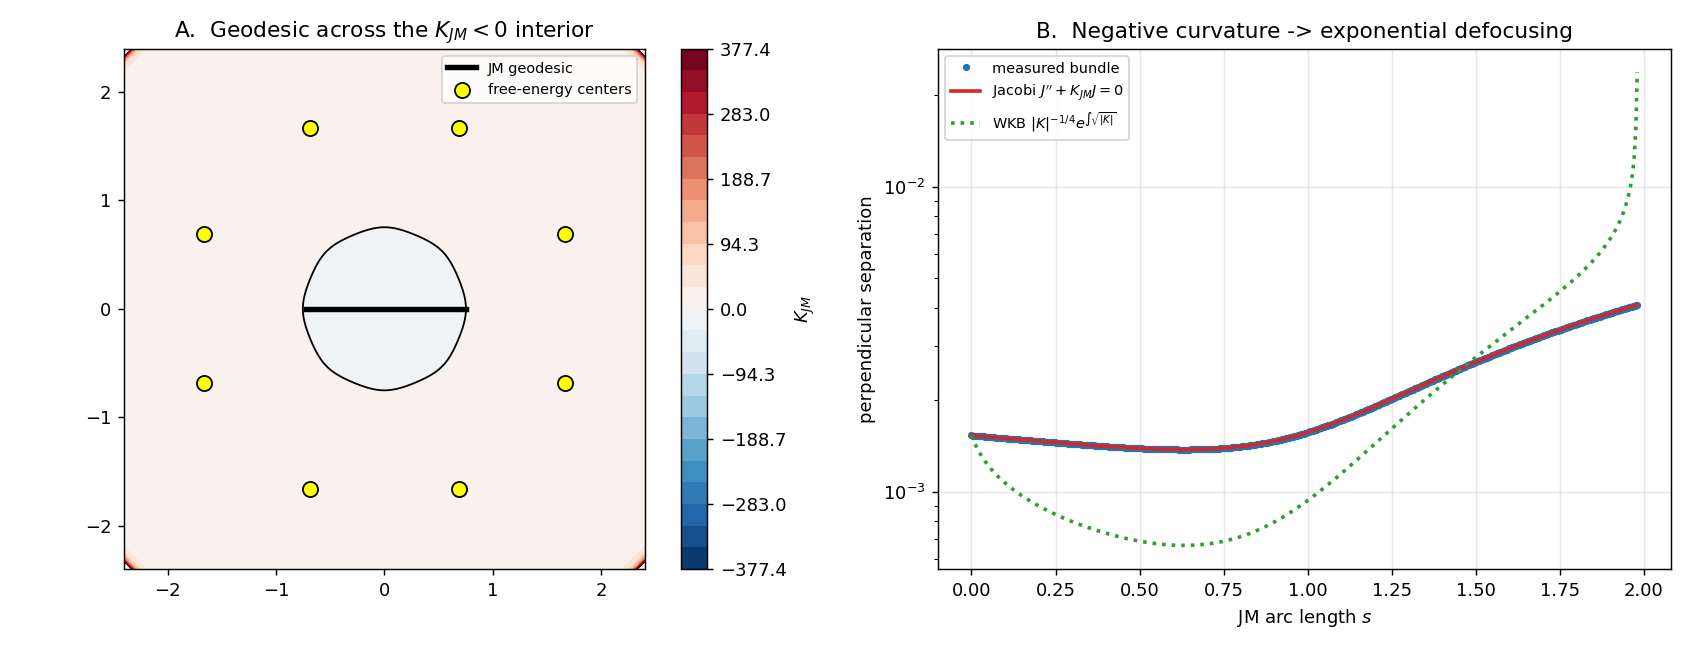
\includegraphics[width=0.92\textwidth]{geodesic_diagnostic.png}
  \caption{Geodesic verification of the Jacobi--Maupertuis curvature.
  \emph{Left:} the curvature field $K_{JM}$ over a synthetic free-energy
  landscape (ring of eight component centres); the reference geodesic
  traverses the negative-curvature interior. \emph{Right:} perpendicular
  separation $\eta$ of a geodesic bundle versus arc length $s$, on a
  logarithmic scale. The separation measured directly from the geodesic
  pair (markers) and the solution of the Jacobi deviation equation
  $\eta''+K_{JM}\eta=0$ driven by the derived curvature (solid) coincide
  to a maximum relative deviation that rounds to $0.00\%$ at the reported
  precision --- agreement to within the integration tolerance. The WKB
  envelope $|K_{JM}|^{-1/4}\exp\!\int\!\sqrt{|K_{JM}|}\,ds$ (dotted) is
  shown for reference. Independently, the closed-form curvature formula
  \eqref{eq:gap:KJM} matches a direct finite-difference evaluation of
  $-\Delta(\log h)/(2h)$ to a median relative error of
  $3.7\times10^{-4}$; this residual is the second-order truncation error
  of the finite-difference stencil and decreases under grid refinement,
  not a discrepancy of the formula. The non-monotone profile --- mild
  contraction near the boundary where $K_{JM}\to0$, then exponential
  defocusing in the curvature well, net amplification $2.7\times$ --- is
  reproduced by the deviation equation across its entire length.}
  \label{fig:jacobi}
\end{figure}

\subsection{Empirical validation on a trained transformer}
\label{sec:gap:empirical}

The verification of Section~\ref{sec:gap:numerics} was synthetic: the
cluster geometry was constructed to exhibit a gap.  A sharper question is
whether the gap-regime occurs in a \emph{trained} network, where nothing
enforces it.  We therefore instrumented a Llama-3.2-1B model~\cite{grattafiori2024llama}
($16$ layers, $32$ heads, head dimension $D=64$) and captured, for every
attention head at every layer, the post-rotary keys, the softmax weights of
each query, and hence the Hessian $H=-\beta\operatorname{Cov}_p(k)$ with
$\beta=D^{-1/2}$ the scaled-dot-product temperature.  Eigenvalues were
computed in single precision.  The corpus was WikiText-2~\cite{merity2017pointer}; three context
lengths $N_{\mathrm{kv}}\in\{512,2048,8192\}$ were measured, yielding
$46{,}080$ head-positions in total.  This is a single model on a single
corpus, and the conclusions are stated with that scope.

\paragraph{Genuine gaps are the rule, not the exception.}
The gap must be assessed by a scale-free criterion: the relative gap
$\Delta(H)/|\lambda_{\max}(H)|$, since the spectral scale itself varies
across layers and context lengths and an absolute threshold would be
miscalibrated.  Using $\Delta/|\lambda_{\max}|>0.05$ as the genuine-gap
test, $96\%$ of all head-positions are in the gap-regime, and the figure is
essentially independent of the threshold over $[0.05,0.1]$.  Restricted to
layers~$1$ through~$15$ the fraction rises to $97\text{--}98\%$.  The
gap-regime --- the precondition under which $\dim E_-$ is a well-posed
invariant (Proposition~\ref{prop:gap:wellposed}) --- is thus not a
synthetic artefact; it is the typical state of attention in a trained
transformer.

\paragraph{An explosive phase transition at the first layer.}
Stratifying by layer reveals a sharp structure.  The input layer~$0$ is
\emph{pre-cluster}: its median gap is small ($\Delta\approx0.5$) and a
large fraction of its heads show no gap at all.  Between layer~$0$ and
layer~$1$ the median gap jumps by an order of magnitude --- to
$\Delta\approx6$ --- and then varies only mildly across layers~$2$--$15$
(the ratio of the layer-$1$ median to the layer-$2$--$15$ plateau mean is
$0.78\text{--}0.86$ across the three context lengths).  The dispersion of
$\Delta$ shows the same jump.  The geometry is therefore not built
gradually through a representational hierarchy; it appears in a single step
at the first layer and is merely refined thereafter.  This is consistent
with the interpretation of layer~$0$ as operating on raw token embeddings,
before the network has assembled the contextual clusters that the
free-energy picture describes: where the precondition fails, it fails for a
structural reason, and it fails in exactly one identifiable place.

\begin{figure}[t]
  \centering
  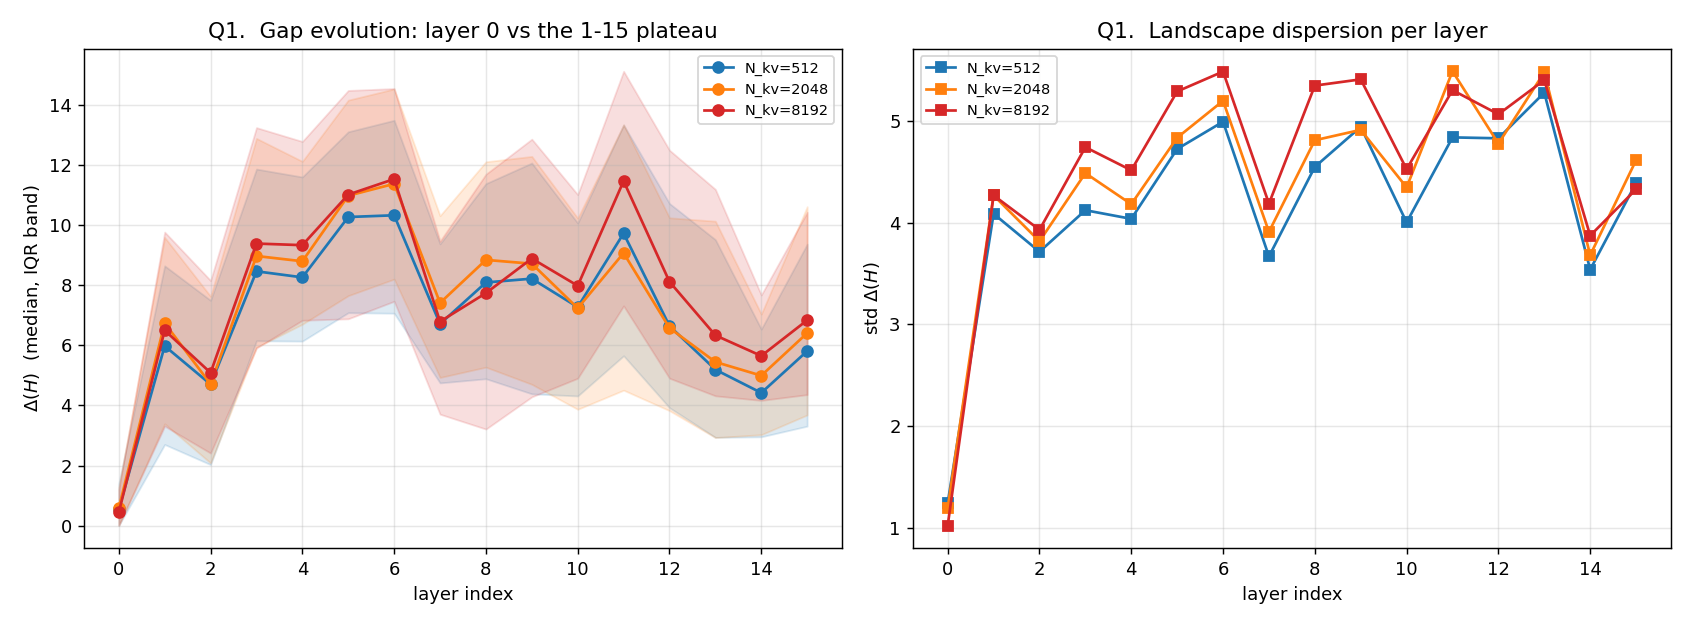
\includegraphics[width=0.92\textwidth]{layer_evolution.png}
  \caption{Layer-stratified gap evolution on a trained Llama-3.2-1B,
  three context lengths. \emph{Left:} the median spectral gap
  $\Delta(H)$ jumps by an order of magnitude between the input layer~$0$
  and layer~$1$, then plateaus --- an explosive phase transition, not a
  gradual hierarchy. \emph{Right:} the dispersion of $\Delta(H)$ shows the
  same jump. The pre-cluster input layer is the one identifiable place
  where the gap-regime precondition fails.}
  \label{fig:layer}
\end{figure}

\paragraph{One dominant mode.}
Among genuine-gap heads, $96\text{--}98\%$ in layers~$1$--$15$ have
$\dim E_- = 1$: a single dominant defocusing mode.  The fraction of such
``clean single-mode'' heads jumps from $0.42$ at layer~$0$ to $0.95$ at
layer~$1$ and holds across the remaining layers.  The naive count can also
saturate at $\dim E_- = D-1$; this is not a rich multi-cluster structure
but the counter running out of dimensions when no gap exists, and it occurs
almost exclusively in layer~$0$.  A guard against this saturation --- reading
$\dim E_- \approx D-1$ as ``no gap'' rather than ``many clusters'' --- is
necessary for any spectral diagnostic, and is recorded as a known
failure mode.  The practical picture of a trained attention head is thus
simple: one strongly-negative transport direction, cleanly separated from a
near-zero bulk.

\paragraph{Scope and the routing signal.}
Two limitations are stated plainly.  First, the rank-local dispatcher of
Section~\ref{sec:multiaxis} routes on the participation ratio of the
\emph{query} covariance $\operatorname{Cov}(Q)$, a different object from the
softmax-weighted key covariance $\operatorname{Cov}_p(k)$ of the theory; on
this corpus the two are statistically uncorrelated (Spearman
$|\rho|\lesssim0.25$ at every layer), so the dispatcher signal does not
track the spectral gap.  This is consistent with the synthetic finding that
the participation ratio is gap-blind.  Second, because gap-closure is
confined almost entirely to layer~$0$, this corpus cannot test the regime
$\Delta\to0$ on the deeper layers; whether corpora with heavier repetition
(code, structured data) populate that regime more is left open.  Neither
limitation weakens the central empirical result: on a trained transformer
the gap-regime precondition holds for the overwhelming majority of attention
heads, it is established by an explosive transition at the first layer, and
the typical head carries exactly one dominant mode.

\subsection{Summary}
\label{sec:gap:summary}

The negative subspace $E_-$ of the free-energy Hessian is a topological
invariant --- threshold-free via the Riesz projector
(Proposition~\ref{prop:gap:wellposed}), perturbation-stable via Davis--Kahan
(Proposition~\ref{prop:gap:dk}) --- exactly inside the gap-regime
$\Delta(H)>0$. The three operating windows of the earlier sections are the
separation, temperature, and energy sections of this one condition. The link
from the invariant to transport instability requires, in addition, the energy
window $E>E^\star$ of \eqref{eq:gap:Estar}; with both conditions in force,
$\dim E_-$ equals the number of exponentially defocusing geodesic directions
and equally the number of unstable modes of the inertial flow, at the rates
$z_+$ of the characteristic polynomial. This is the spectral foundation on
which the adaptive rank-local routing of Section~\ref{sec:multiaxis} rests:
the router's effective rank $r^\star$ is well-defined precisely when
$\Delta(H)>0$, and the regime $\Delta\to0$ is the structural --- not
numerical --- signature of the transition to the dense regime.
Section~\ref{sec:gap:empirical} confirms that this foundation is not merely
synthetic: on a trained Llama-3.2-1B the gap-regime holds for $96\%$ of
attention heads, established by an explosive transition at the first layer,
with the typical head carrying exactly one dominant mode.


% =====================================================================
\section{Related work}
\label{sec:related}

\paragraph{Geometry of the space of measures.}
The picture used here --- a free-energy functional whose Wasserstein
Hessian governs the stability of a transport flow --- sits in the
Otto-calculus tradition. Otto's formal Riemannian structure on the space
of probability measures~\cite{otto2001geometry} and the variational
(JKO) formulation of diffusion~\cite{jordan1998variational} established
that gradient flows of free energy are geodesic-type objects;
Ambrosio, Gigli and Savar\'{e}~\cite{ambrosio2008gradient} and
Villani~\cite{villani2009optimal} give the rigorous metric theory. The
Brenier polar-factorization theorem~\cite{brenier1991polar} is what makes
the static transport map a $W_2$ object. Lott and
Villani~\cite{lott2009ricci} connect displacement convexity to a
synthetic Ricci-curvature bound; the present paper's Jacobi--Maupertuis
curvature and its sign condition are a finite-dimensional, attention-
specific instance of that displacement-curvature circle of ideas. Our
contribution is not the geometry itself but the spectral
\emph{well-posedness} question --- when the negative-eigenvalue count is
an invariant --- which the metric-geometry literature does not address
because it works with the full operator rather than an integer count.

\paragraph{Spectral perturbation theory.}
The two technical pillars are classical. The Riesz projector and the
analyticity of spectral subspaces are from Kato's perturbation
theory~\cite{kato1995perturbation}; the stability of an invariant
subspace under a perturbation small relative to the spectral gap is the
Davis--Kahan $\sin\Theta$ theorem~\cite{davis1970rotation}. The present
paper applies them not to a numerical-linear-algebra problem but to the
free-energy Hessian of attention, where the gap acquires a mechanistic
meaning: it is exactly the condition under which the transport-instability
count is physical.

\paragraph{Attention and efficient transformers.}
Attention~\cite{vaswani2017attention} is treated here as one instance of a
free-energy potential; the LogSumExp form is the bridge. On the systems
side, FlashAttention~\cite{dao2022flashattention} and its decode variants
established the streaming-from-HBM pattern that the $\Phi$-Transport
router builds on. The empirical study is on
Llama-3.2-1B~\cite{grattafiori2024llama} over
WikiText-2~\cite{merity2017pointer}. This paper does not propose a new
attention mechanism; it supplies the spectral foundation under an existing
adaptive router, and asks whether the geometry that foundation predicts is
actually present in a trained model.

\paragraph{Attention as optimal transport.}
The view of attention as a transport process has an established line.
Daneshmand~\cite{daneshmand2024provable} shows that softmax self-attention
layers can simulate gradient descent on the dual of the
entropy-regularized optimal-transport problem, with transformer depth
controlling the approximation accuracy. Litman~\cite{litman2025sdpa}
proves that the scaled-dot-product attention forward pass is the exact
solution of a one-sided entropic optimal-transport problem, and --- most
relevant here --- analyses the \emph{information geometry} that this
formulation induces on the space of attention distributions, via the
Fisher information matrix. The present paper shares the premise that
attention is a transport process, but its object is different. Those works
study the transport \emph{map} (the attention weights themselves) and the
geometry of the \emph{distribution simplex}; we study the Hessian of the
free-energy potential \emph{with respect to the query position}, and the
geometry of the \emph{query configuration space} through the
Jacobi--Maupertuis metric. The Fisher geometry of
Litman~\cite{litman2025sdpa} lives on the output simplex; our
Jacobi--Maupertuis geometry lives on the input domain. They are
complementary descriptions of the same mechanism from opposite ends.

\paragraph{Hessian eigenvalues and spectral gaps in transformers.}
Two neighbouring uses of spectral language must be distinguished from ours
explicitly, since the words coincide while the objects do not. First, the
\emph{loss-function Hessian}: negative eigenvalues of the training-loss
Hessian of deep networks have been studied since
Sagun et al.~\cite{sagun2016eigenvalues}, who identified the
bulk-plus-outliers spectral structure, and Alain et
al.~\cite{alain2019negative}, who examined the role of the negative
eigenvalues directly. That Hessian is taken with respect to the
\emph{model parameters} and describes the optimisation landscape; ours is
taken with respect to the \emph{query position} and describes a transport
landscape at a fixed, trained model --- a different operator on a different
space, and the negative-eigenvalue count means a different thing. Second,
the \emph{attention-matrix spectral gap}: Nait Saada et
al.~\cite{naitsaada2025mindthegap} analyse the gap between the two largest
singular values of the attention matrix itself, and identify it as the
driver of rank collapse. That gap is a property of the row-stochastic
attention matrix; ours is a property of the free-energy Hessian
$H=-\beta\operatorname{Cov}_p(k)$, a symmetric negative-semidefinite
operator. The two are not the same spectral object: theirs separates
signal-propagation modes of a Markov matrix, ours separates the
transport-instability subspace of a curvature operator. We adopt the term
``spectral gap'' in its standard operator-theoretic sense and flag the
coincidence to forestall confusion.

% =====================================================================
\section{Conclusion}
\label{sec:conclusion}

The negative subspace of the free-energy Hessian is the object on which
the $\Phi$-Transport router rests, and this paper has shown when that
object is mathematically well-defined: exactly inside the gap-regime
$\Delta(H)>0$. Inside it, $\dim E_-$ is threshold-free (the Riesz
projector) and perturbation-stable (Davis--Kahan); the framework's three
empirical windows are one spectral condition seen from three coordinate
axes; and the link to geometric defocusing holds under one additional,
precisely-stated energy restriction. The measurement on a trained
Llama-3.2-1B closes the argument: the gap-regime is not a property of
hand-built synthetic geometry but the ordinary state of attention in a
working transformer, reached by an explosive transition at the first
layer, with the typical head carrying exactly one dominant transport
mode. The router's effective rank is therefore a well-posed quantity in
the regime where the router operates --- and the regime $\Delta\to0$, far
from being a numerical nuisance, is the structural signature of the
transition to dense attention.

% =====================================================================
\bibliographystyle{plain}
\bibliography{refs}

\end{document}
